% Shared standalone design for the editable figure reconstructions.
\documentclass[tikz,border=5pt,10pt]{standalone}
\usepackage[T1]{fontenc}
\usepackage[utf8]{inputenc}
\usepackage{newpxtext,newpxmath}
\usepackage[scaled=.94]{sourcesanspro}
\usepackage{pgfplots}
\pgfplotsset{compat=1.18}
\usetikzlibrary{arrows.meta,calc,positioning,decorations.pathreplacing,
  decorations.markings,patterns,matrix,shapes.geometric,fit,backgrounds,
  intersections,angles,quotes}
\definecolor{ink}{HTML}{203746}
\definecolor{accent}{HTML}{146C78}
\definecolor{muted}{HTML}{667780}
\definecolor{signalred}{HTML}{B94B44}
\color{ink}
\tikzset{>=Latex,line width=.8pt,
  every node/.style={font=\small},
  axis/.style={->,draw=muted,line width=.5pt},
  guide/.style={draw=muted,dashed,line width=.45pt},
  curve/.style={draw=accent,line width=1pt},
  marker/.style={circle,fill=accent,inner sep=1.5pt},
  labelbox/.style={fill=white,inner sep=2pt}}

\begin{document}
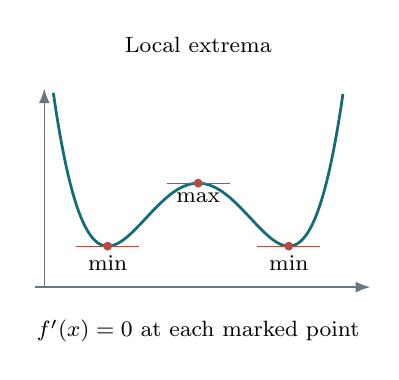
\begin{tikzpicture}[x=1.15cm,y=.8cm,every node/.style={font=\footnotesize}]
\draw[axis] (-1.8,0)--(1.9,0);\draw[axis] (-1.7,0)--(-1.7,3.15);
\draw[curve,domain=-1.6:1.6,samples=180] plot (\x,{((\x)^2-1)^2+.65});
\foreach \x/\y/\lab in {-1/.65/min,0/1.65/max,1/.65/min}{\draw[signalred] ({\x-.35},\y)--({\x+.35},\y);\fill[signalred] (\x,\y) circle(1.6pt);\node[below] at (\x,\y) {\lab};}
\node at (0,3.85) {Local extrema};\node at (0,-.7) {$f'(x)=0$ at each marked point};
\end{tikzpicture}
\end{document}
